\input{preamble}
\makeglossaries

%----------------------------------------------------------------------------------------
\input{sections/definitions}

\begin{document}
\setlength{\abovedisplayskip}{1cm}
\setlength{\belowdisplayskip}{.8cm}

\includepdf{sections/forside}

%\newpage\null\thispagestyle{empty}\newpage
%----------------------------------------------------------------------------------------
%	FRONTMATTER
%----------------------------------------------------------------------------------------
\frontmatter

%Abstract

\begin{abstract}
This master's thesis seek to investigate some of the common approaches used for \ab{NILM}, in order to determine the capabilities and limits. It is assumed that the \ab{NILM} application is deployed in a modern smart grid. The impact the smart grid infrastructure have on the data quality is investigated. It is shown that equipment and network errors are the major quality decreasing factors. Simple gap filling methods are evaluated in order to improve the quality. It is shown that simple gap filling can improve the performance. The performance is also shown to be depended on the number of appliances that are in a given environment, and the consumption requirements of the appliance. Interference from other appliances have a major effect on the performance. Higher sample rates and norm filters is shown decrease the interference. In general is an acceptable performance only obtained on the top consumers in the household. A small case study illustrates how a \textit{service provider} in a smart grid can benefit from the information collected with a \ab{NILM} application.
\end{abstract}


%Danish Abstract

\renewcommand{\abstractname}{Resumé}
\begin{abstract}
Dette speciale undersøger mulighederne og begrænsningerne med \ab{NILM}. Kvaliteten der kan forventes af data modtaget i en moderne smart grid infrastructure undersøges. Det er vist at fejl i måleudstyr og servere er nogle af de store kvalitets dæmpende aspekter. Forskellige ”Gap filling” metoder er undersøgt, for at udbedre fejlene, og øge kvaliteten. Det er vist at simple ”Gap filling” metoder kan øge kvaliteten. Det er vist at resultatet af \ab{NILM} bliver væsentligt forringet hvis der er mange apparater i det samme miljø. Energikravene for de enkelte apparater har også meget at sige for resultatet. Interferens fra andre apparater er med til at forringe resultatet af \ab{NILM}. Det er vist at højere sample hastigheder vil kunne og ”norm filtre” vil kunne forbedre resultaterne markant. Generelt er det kun de apparater der bruger mest energi i husstanden, der får acceptable resultater. Et lille brugsscenarie viser hvordan en \textit{service provider} kan benytte informationer fra \ab{NILM} applikationer til at udvide deres forretningsmuligheder. 


\end{abstract}

\chapter*{Preface}
This is a master's thesis of M.Sc in computer technology by Rune Arbjerg Heick. The work and writing to the thesis is conducted in the period September 2015 to April 2016. The theme of capability and limits of non-intrusive load monitoring is found in collaboration with Rune
Hylsberg Jacobsen and Emad Samuel Malki Ebeid. It is the hope that techniques and approaches investigated in this work can help support their continued research in the field.

\section*{Reader's Guide}
Through the report, references are made according to the IEEE standard. A bibliography is added at the end of the report. All citations are numbered in the order they are mentioned. Figures, tables and equations are numbered corresponding to the chapter and a sequential number indicating the order the item is in the chapter E.g. Figure 1.3 is the third figure in chapter one.  

All abbreviations is spelled out at first occurrence in each chapter. A list of abbreviations is also included in the beginning of the report. All special definitions is marked with quotation marks at first occurrence in the report. A small description is given at first occurrence, and in the definitions overview in the beginning of the report. All other occurrences is illustrated by italic. Quotation marks is also used at direct and indirect citations or as naming illustrator. 

All appendixes supplied with this report is digital and a link to the online location can be found in the appendix overview, at the end of the report.  

\section*{Acknowledgments}
A special thanks to Rune Hylsberg Jacobsen and Emad Samuel Malki Ebeid for taking the time of giving feedback and improve the thesis project. Thanks to the SmartHG project for allowing access to the Danish SmartHG dataset and thanks to ETH Zurich for providing the ECO dataset. 

% Glossary and Abbreviations
%----------------------------------------------------------------------------------------
\printglossary[type=\acronymtype,title=Abbreviations,nonumberlist] % prints just the list of acronyms

\printglossary[nonumberlist] % if no option is supplied the default glossary is printed.
\newpage

% List of Figurs/Tables
%----------------------------------------------------------------------------------------
{%
\let\oldnumberline\numberline%
\renewcommand{\numberline}{\figurename~\oldnumberline}%
\listoffigures%
}
\vspace{10mm}
{%
\let\oldnumberline\numberline%
\renewcommand{\numberline}{\tablename~\oldnumberline}%
\listoftables%
}

% TOC
%----------------------------------------------------------------------------------------
\newpage
\tableofcontents

%----------------------------------------------------------------------------------------
%	MAINMATTER
%----------------------------------------------------------------------------------------
\mainmatter

%2 pages
\resetAcr
\chapter{Introduction}
In the past electricity production and consumption was localized to small communities. The communities often had one electricity utility company supplying the required energy. As the energy demand increased beyond single production facilities, the solution was to add more production facilities that could support in peak hours. This approach is costly, since such support facilities must be kept in a standby state, ready to deliver additional energy at a moment’s notice~\citep{RefWorks:46}. As the electric grid expanded, it began to interconnect the communities. The distribution of energy in the grid also became a challenging task. Today's electricity grids are a more global grid that span many communities, and even countries. The consumer plays a passive part in the grid. It is the operators of the electricity grid that must ensure that energy is delivered at the different consumers, at correct quantities, without overloading the grid. Furthermore must the impact errors and damages have on the grid be minimized~\citep{RefWorks:43}.

\section{smart grid}
In order to combat some of the problems in the grid today, is a new type of electricity grid being deployed. As sensor technology became cheaper and more reliable the electricity utility companies started to integrate sensors in the grid. These sensors delivered information about the performance of key sections of the grid. This information was used to improve the performance of the grid. More types of energy producing devices, such as solar power and wind turbines, got connected to it. This created a need for more control of the grid and the energy production. This laid the foundation for the new grid type called smart grid~\citep{RefWorks:43}.

The \ab{NIST}[National Institute of Standards and Technology] is tasked with the job of creating and maintaining the standards used for the American smart grid. The concept behind the smart grid is to create an electricity grid that enables two way communication. Besides electricity must information about the usage also flow between the consumers and the utility companies. Usage patterns must flow to the engineers tasked with controlling the grid, and control information must flow back to the consumers or control points in the grid. This can ensure the delivery of electricity more efficiently, reliably, and securely ~\citep{RefWorks:42}. 

There are many different kind of stakeholders in today's smart grid. In order to better understand the needs and relationships between the stakeholders have \ab{NIST} split them in to seven domains. This helps to identify the different user interest in the grid, and their needs.  

\newpage % for nice page formatting 

\begin{figure}[H]
\centering
\includegraphics[width=1\textwidth]{billeder/SMARTGRID.png}
\caption[Conceptual model of smart grid architecture.]{Conceptual model of smart grid architecture. Source~\citep{RefWorks:41}}
\label{fig:CMOSG}
\end{figure}
 
Figure~\ref{fig:CMOSG} illustrates the seven domains. The seven domains each have a set of functions that is characteristic for the domain~\citep{RefWorks:41}.  
 
\begin{tabularx}{\linewidth}{ r X }
Generation:& The \glsreset{generator}\df{generator} role is the generators of electricity. This is typically coal, oil or nuclear power plants or large-scale hydro generators. This can also include energy storage facilities that stores energy for later distribution. \\\\

Transmission:& \glsreset{transmission}\df{transmission} and transformers that hold the purpose of transporting the electricity over large distances. \\\\

Distribution:& The \glsreset{distribution}\df{distribution} role are the units responsible of electricity distribution to and from the customers. \\\\

Customer:& The \glsreset{customer}\df{customer} role is the consumers of electricity. They may also generate electricity and sell it to the grid. \\\\

Operator:& The \glsreset{operator}\df{operator} role is managers of the movement and production of electricity. They are the group that ensures that the energy is efficiently delivered where it is needed. \\\\

Market:& The \glsreset{markets}\df{markets} is the instance responsible for sale and purchase of electricity between the different instances of the grid. Not just the \df{customer} uses this instance. Utility company can also purchase power from each other to keep up with demand at peak hours. \\\\
\end{tabularx}
\begin{tabularx}{\linewidth}{ r X }
Service Provider:& The \glsreset{service provider}\df{service provider} role are the organizations providing services to the utility companies or the \df{customer}. This could be home automation or information services.  \\
\end{tabularx}

\section{Non-Intrusive Load Monitoring}
The \df{operator} have the responsibility of controlling the flow of energy on the smart grid. This requires the knowledge of the current consumption and a prediction about the future power requirement. This prediction is generality based on statistical data collected in the grid. If the prediction of the future power requirements can be improved, it is possible to create a better and more efficient power distribution. To accomplish this is a method known as \ab{NILM} developed.

The concept of \ab{NILM} is to use the consumption information collected at household level, and use machine learning techniques to make a qualified guess on what appliances in the household is responsible for the current consumption. By using the information from the active appliances more precise estimates of future consumption can be made. 

In today's smart grid are all \df{customer}\textit{s} equipped with smart meters. The smart meter measures the consumption of the household, and reports it back to the smart grid. This information can be used by the \df{markets} to automatically create billing information, or by the \df{operator} to regulate the power distribution. Since this information is used for distribution regulation it is send in real-time~\citep{RefWorks:41}. It is this information \ab{NILM} applications hopes to use in order to create better predictions.

\ab{NILM} can also create many opportunities for the \df{service provider}. Using \ab{NILM} it is potentially possible to gesture about the usage of each appliance in a household. This can be used to better inform the resident about power saving opportunities. Studies have shown that detailed information about energy usage, makes the resident use less energy~\citep{RefWorks:33}. Other business opportunities, like selling the statistical information about the usage of specific appliances might also exists.  

\section{The Problem Statement}

This master's thesis seek to investigate some of the common approaches used for \ab{NILM} today, in order to determine the capabilities of such approaches. It is assumed that the \ab{NILM} approaches are used in a modern smart grid setting. In order to answer this broad question, the following questions must be investigated. 

\begin{itemize}
\item	\textbf{What quality of data can be expected from a smart meter infrastructure?}\\
In a smart grid is a lot of information collected from various points. For a system that needs the smart meter data to be collected on a server, what quality can be expected? And where in the infrastructure, that collects and transports the information over the Internet, is the quality being compromised? \\
	
	
\item	\textbf{How does sample errors and poor quality affect \ab{NILM} applications?}\\
If the system contains errors, due to samples being lost in the network, how does this impact the \ab{NILM} applications?  Does the quality effect the performance of \ab{NILM} disaggregation? \\
	
\item	\textbf{What behaviours can be detected using \ab{NILM} and where are the limits?} \\
How detailed is it possible to gesture about the behaviour of the appliances in a household? Where are the limits of susses? And what does these limits depend on?  \\
	
\item	\textbf{What can be done to improve the performance of \ab{NILM} technology?}\\
Is it possible to clean data to improve quality and performance? What aspects is the bottlenecks for \ab{NILM} technology today, and how does one improve on this basis? \\

\end{itemize}
If these question is answered it creates a strong foundation for gesturing about the the capability of \ab{NILM}. The main motivation for this study is not to improve grid load predictions, but to get a better basis for validate different \ab{NILM} related business opportunities for \dfs{service provider}.

\section{The Approach}
Research on the popular methods and definitions in various areas of \ab{NILM}, quality and machine learning has been analysed. The result is used to create the basis of the experiments conducted in this master's thesis. In order to investigate the questions in the problem statement is real data needed.

\subsection{The Data Approach}
As dataset is the SmartHG dataset used. The SmartHG dataset is a collection of smart meter data collected from 25 residential households in Denmark. The data is not filtered or cleaned in any way prior usage. This means that the data closely resembles what would be collected in a smart grid. Furthermore does the dataset contain information about the usage pattern of selected devices. This information can be used to compare inferred usage patterns to the actual pattern. 

\begin{figure}[H]
\centering
\includegraphics[width=1\textwidth]{billeder/DataCollection.png}
\caption{Data collection process.}
\label{fig:DCP}
\end{figure}
The data is collected from the houses main meter and sub-meters, by attaching a ZigBee module to the meters. The modules transmits the values from the meter to a ZigBee gateway. The gateway transmits the data over the Internet to a database service in the university. This process is illustrated in Figure~\ref{fig:DCP}.

\subsection{The Experiment Approach}
Some of the experiments are conducted on real data, as it would be observed in a real deployment scenario. The behaviours observed in this types of experiment is used to design a series of experiments in controlled conditions, using artificial constructed datasets. These experiments serves the purpose of exposing the properties responsible for the observed behaviour. This improves the understanding of what properties creates wanted and unwanted behaviour.

% 6 pages
\resetAcr 
\chapter{Data Quality}
Various projects today is focused on gathering data and analysing it. The gathered data is used for obtaining behaviours, habits and properties of the observed objects. This is done by using powerful statistical leaning algorithms, that are able to deduce these properties from the data. This approach is called data driven development, since the success is mainly determined by the data and not the algorithm. 

When data is the central role of the system, the quality of the data are very important. Poor data can let to wrong assumptions, and have a negative effect on the application. Choosing the correct dataset is therefore a key factor \cite{RefWorks:3}. Looking at the quality of the data can help you chose what dataset to use. Data quality can be described many ways, one of the more formal is from the ISO 8402 standard that describes quality as: 

\begin{adjustwidth}{2.5em}{2.5em}
\emph{"The totality of characteristics of an entity that bear upon its ability of satisfy stated and implied needs"} \cite{RefWorks:5}.
\end{adjustwidth}

This indicate that data quality is something that is very depended on the intended use and is therefore hard to generalize. 

Quality of data is a subject that is gaining more and more attention due to the fact that we are moving data gathering from controlled labs, to the public. Many of these projects is the citizen science project, where it is the citizen who collect the data, and not interested parties \cite{RefWorks:2}. This enables researchers to gather enormous amount of data, but they are no longer in control of the conditions the data is collected in, which introduces errors and other quality decreasing factors. 


\section{Quality Parameters}
It is not uncommon that deficient areas of of research has its own quality criteria. This is due to the fact that quality is a very domain specific subject.

One of the areas that have been dealing with citizen data for many years is the Geographic information area, that are used for maps, weather prediction and climate research. They have come up whit several ways of describing quality in spatial data \cite{RefWorks:7}. Method for defining quality in time series data have also been developed  \cite{RefWorks:6}. 

One of the things all the methods have in common is trying to look at the completeness of the data. Some of the most low level criteria is the sample availability. Here we asses if there is gaps in the data, that is caused of unknown interference, and look at how the samples is distributed in the measurement period.  


\section{Appliance Citizen Data}
As a part of the SmartHG project 25 households have been equipped with meters on selected appliances and the main meter. The data collected from this experiment are are prone with errors due to malfunctioning test equipment or unexpected interference from the resident there have been unintentionally turning off the measurement equipment for a period of time. 

The sample availability quality of the data in the SmartHG dataset have been measured on a hour basis.  The quality for each meter is assessed by looking at the available samples over the maximum expected samples in the period.  
\begin{gather}
		N_{max}^{(m,T)} = \floor{ (\phi_{start}^{(m,T)} - T_{P})\times T_s^{(m)} } \label{EQ:NMAX} \\
		q^{(m,T)} = \frac{N_{observed}^{(m,T)}}{ N_{max}^{(m,T)} } \label{EQ:QMT}
\end{gather}
As shown on equation \ref{EQ:NMAX} is the maximum number of samples for a meter $m$ in the period $T$ calculated by taking the period time $T_P$, corrected with the sample phase $(\phi_{start}$ for the given period, and dividing it with the sample time $T_s$. The quality of the meter is calculated as the ratio of observed samples in the timeslot $T$ to the maximum samples, shown in equation \ref{EQ:QMT}. 

To find the quality of a house in a given period $T$, that have a set of meters $M$, we take the mean value of all the meter quality's, as shown in equitation \ref{EQ:HQT}.  
\begin{equation}
	\mu_{q^{(M,T)}} = \frac{1}{\mathbf{card}(M)} \sum_{m \in M} q^{(m,T)}
	\label{EQ:HQT}
\end{equation}
Each house has a quality vector $Q$, with the house quality found whit a period $T_P$ on one hour. This have been done from April $t_{start}$ to October $t_{end}$. 
\begin{equation}
	Q^{(M,t_{start},t_{end} )} = \{ \mu_{q^{(M,T)}} | T \in \{t_{start}, t_{start}+T_p,t_{start}+2 \times T_p, ... , t_{end}  \} \}
	\label{EQ:HQV}
\end{equation}
This is shown in equation \ref{EQ:HQV} where M is a set of the meters in a given house. This can be graphically shown on the figure \fxnote{show the figure of quality} where the color is a gradient running from light green for the best quality to red for bad quality.   


\section{Related Work}

% 8 pages
\resetAcr
\chapter{Gap Reconstruction}
\label{Sec:GapFill}
One of the more common problems in citizen science projects is gaps in data. This can happen either if the network connection is unstable or the test equipment gets prematurely turn off, as discussed in chapter \ref{Sec:DataQuality}. This can greatly degrade the data quality, and lead to errors in the application. One way to deal with this problem is to use mathematical gap filling techniques to come with a qualified guess on how the data would look like in the gap. 

In order to use this methods we must assume that the missing data in the gap follows the same behaviour as the data on each side off the gap. If the signal is so stochastic that this is not the case then gap filling is not recommended\citep{RefWorks:10}. 

In the case of the SmartHG project the data can be seen to have a part that is depended on the previous and future data plus a stochastic part that are determined by the user and the appliance. Due to the stochastic part a perfect reconstruction is not possible, but it is the hypotheses that the non stochastic part is still so dominant that a decent reconstruction is possible. 

\section{Gap Filling Methods}
\label{T:GapFilling}
Various methods exists for gap filling. Five popular algorithms are selected for this project, and is validated on the SmartHG project data. These methods have been chosen since they all have a different approach on the gap filling process. For some of the algorithms it is important to keep the frequency spectra as intact as possible, for other it is the jitter power or the exact sample value they are trying to estimate. Some algorithms have also been designed for small gaps, while others have been designed for larger. 

In the following sections it will be briefly described what makes the five algorithms unique, and how they work. 

\subsection{Papoulis-Gerchberg Algorithm}
\label{T:PGA}
The \ab{P-G}[Papoulis-Gerchberg] algorithm is a multi gap filling algorithm, meaning it is capable of correcting more than one gap at the time. This makes the algorithm preform good in conditions with many gaps and few available data points between gaps. This is due to its ability to collect information about the signal across multiple gaps\citep{RefWorks:11}. The \ab{P-G} algorithm works under the assumption that the signal is a periodic stationary signal with a known bandwidth. The signal will therefore consist of $M$ frequency components, and everything outside the band is assumed to be noise. The signals in the SmartHG is not stationary, but for small snippets can approximately stationariness be assumed. 

The true bandwidth is also unknown in the signal. The \ab{P-G} algorithm is very depended on the bandwidth for a correct reconstruction. A modified version of the algorithm that estimates the bandwidth, by varying the frequency components $M$ and analysing the mean square error on the known signal is therefore used \cite{RefWorks:13}. This approach is fairly good at estimating the true value of $M$, but it is time-consuming.

\subsection{Wiener Filling Algorithm}
The Wiener filling algorithm is an extension of a Wiener predictor, the Wiener predictor assumes that there exist a linear relationship between the next sample and the previous samples. By trying to predict the missing samples from both sides of the gap, and combining the knowledge, it estimates the missing samples \citep{RefWorks:14}. For larger gaps does this methods rely on earlier predictions to close the gaps. This result in errors being accumulated over the gaps. The method is fast, and is therefore suited for large data with small gaps. 

\subsection{Spatio-Temporal Filling Algorithm}
The \ab{SSA}[Spatio-Temporal filling] algorithm uses singular spectrum analysis to split the signal into a series of sub-signals. The sum of the sub-signals is the original signal, and the sub-signals are ordered so the most dominant is first, and the least dominant is last. 

The reconstruction philosophy is that the gap has introduced noise in the signal, but a sum of only the most dominant sub-signals must be close to the original signal without noise. But in order to know how many sub-signals to include in this sum, we introduce an other artificial gap. While the sub-signals are being accumulated the mean square error of the artificial gap is observed. When this mean square error hits its minimum peek, it is assumed that the reconstruction is as good as possible \cite{RefWorks:15}.

This method is very popular for gap filling. It has shown to be very noise resistant since it finds the overall trends in the data. It does require quite a lot of data to be known post and prior to the gap since an artificial gap must be introduced. It is based on singular spectrum analysis which assumes that the signal consist of stationary processes. This is a similar constraint to the \ab{P-G} Algorithm in section \ref{T:PGA}.

\subsection{Envelope Filling Algorithm}
\label{T:EGA}
Unlike the previous described methods does the Envelope filling algorithm not depend on frequency analyses, but rather on the expected power of the signal. Looking at the envelope of the signal it assumes that all local maxima and minima must lie on the  upper and lower envelope. It then looks at the data prior and post the gap and try to estimate the number of local maxima and minima in the gap, and their locations. It does this by looking for patterns in the time series data \citep{RefWorks:6}. When the new maxima and minima are found the points is connected by using spline \cite{RefWorks:16}. 

The methods do not make any assumptions about the signals stationariness or bandwidth. The method can also be used on none equally spaced time series. 

\subsection{Empirical Mode Decomposition Filling Algorithm}
The \ab{EMD}[empirical mode decomposition filling] algorithm uses empirical mode decomposition, to break the signal into \ab{IMF}[intrinsic mode functions]. The sum of all \ab{IMF}'s is the original signal. The \ab{IMF}'s is all more low frequent and simpler in structure than the original signal. The hypothesis is that it is easier fixing a gap in a simple signal than a complex one. 

The envelope filling algorithm in section \ref{T:EGA} is used to fix the gaps in the \ab{IMF}'s. The \ab{IMF}'s can now be accumulated to get the original fixed signal. Like the envelope filling algorithm does it not make any assumptions about the signals stationariness, bandwidth and can be used on none equally spaced time series. But making a empirical mode decomposition on a signal with a gap in is a non trivial process and can introduce errors \citep{RefWorks:16}. 



\section{Gaps In SmartHG Dataset}
The gaps in the SmartHG project dataset is caused by a lot of different sources such as bad network connection, unplugged measurement equipment or server breakdown. This makes the type of gaps different from case to case. Three aspects of a gap is important for the gap filling: The size of the gap, the data known before the gap, and the data known after the gap. 

\subsection{Gap Size}
On figure \ref{fig:GapSize} is the quantity of different gaps shown. The different gap size is measured as samples missing, e.g. a gap size on 3 means that there is 3 samples missing in a row, between two received samples. Looking at the different gaps in the dataset we see that the normal gap is relatively small. Most of the gaps are between 1-5 samples as seen figure \ref{fig:GapSize}.

\begin{figure}[H]
\centering
\begin{minipage}{.3\textwidth}
  \centering
  \includegraphics[width=1\linewidth]{billeder/GapInfo1.png}
  \captionof{figure}{Gap quantity}
  \label{fig:GapSize}
\end{minipage}%
\begin{minipage}{.8\textwidth}
  \centering
  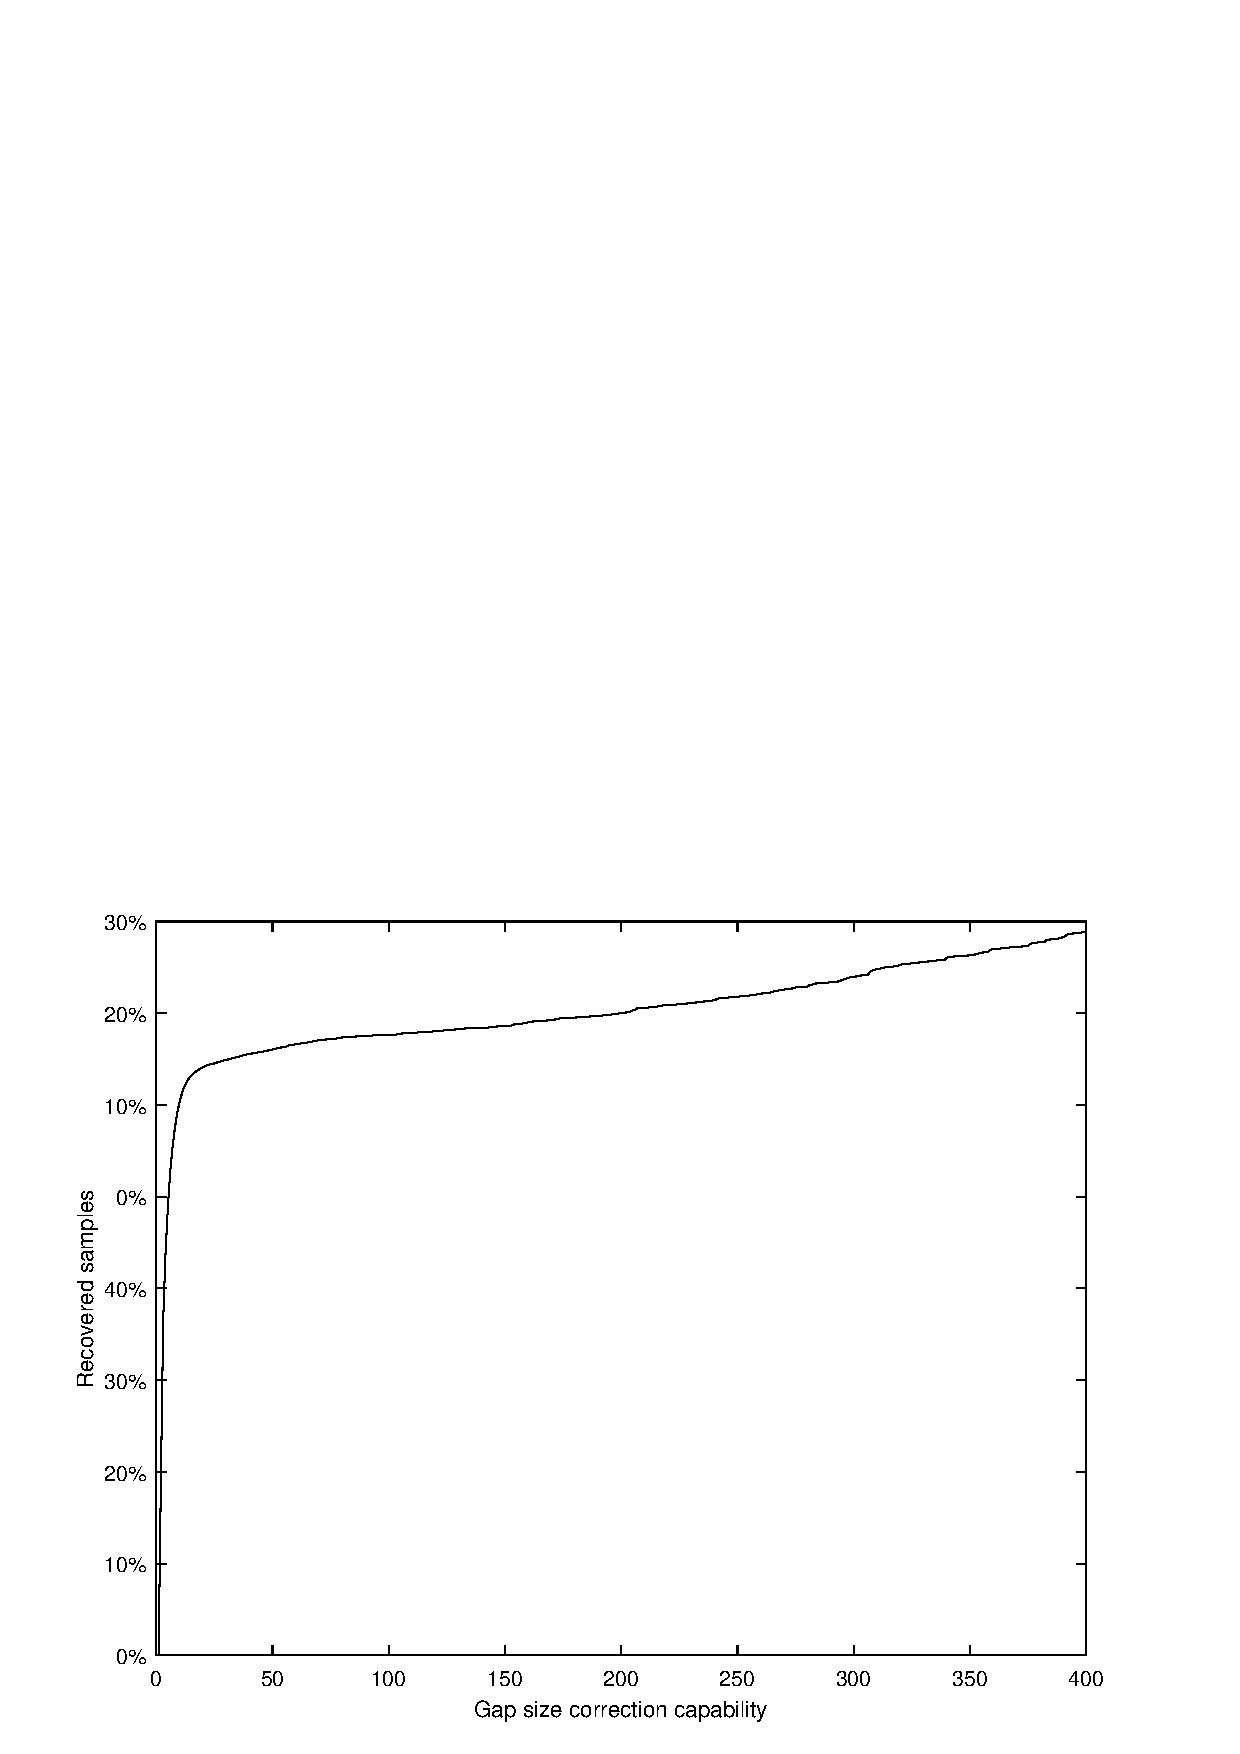
\includegraphics[width=0.8\linewidth]{billeder/CorrectionCapability.png}
  \captionof{figure}{Error recovery capability}
  \label{fig:GapCorrect}
\end{minipage}
\end{figure}

The aim of data reconstruction is to recover the missing samples. The gap size correction capability is a metric telling how big gaps it is possible to correct. If a application has a gap size correction capability on 5 it means that is is capable of correcting gaps that have the gap size of 5 samples or smaller. 

On figure \ref{fig:GapCorrect} is shown how much of the missing signal that can be reconstructed with different gap size correction capability. It is shown that a if a gap size correction capability of approximately 20 samples can be achieved, it is possible to recover $30\%$ of the missing data in the SmartHG dataset. Since the signal is partly stochastic, and it is not possible to recover the stochastic part, the complete signal can newer be reconstructed. The greater the gap, the greater influence does the stochastic part have on the signal. Smaller gaps can therefore be fixed with greater success. It is therefore unlikely that recovery of more than $30\%$ will be possible. 

\subsection{Post And Prior Knowledge}
The reconstruction process works by looking at the samples available prior and post of the gap. Common for all reconstruction methods is that they assume that the signal in the gap must have behaved in relation to the samples prior and post for the gap. Therefore is the samples prior and post for the gap called knowledges, since it grants the knowledges used for reconstructing the gap. 

But in a signal with lots of gaps it can be interesting to see how much knowledge is available for reconstructing a gap. This is done by seeing how many samples that are available prior and post to the gap. This is important since much data allows for detailed models, that can improve gap reconstruction and little knowledge gives the stochastic part dominance which will lead to error prone reconstruction. 

\begin{figure}[H]
\centering
\includegraphics[width=0.7\linewidth]{billeder/GapInfo2.png}\caption{Available samples for recovery}
\label{fig:PAF}
\end{figure}

In the case of the SmartHG project dataset the data available prior and post to a gap varies greatly but is around the same max and min values for every gap size. The median samples available to fix a gap is around 6 samples as shown in figure \ref{fig:PAF}. On the figure is shown that no matter the gap size is the expected knowledge about the same. This can be problematic since lager gaps offend needs more knowledge than smaller gaps. This further indicates that complete recovery of all gaps is impossible. 

\section{SmartHG Dataset Reconstruction}
The data reconstruction algorithms mentioned on section \ref{T:GapFilling} have been tied on the SmartHG dataset. First have 6 unique error free areas in the data been found, and a artificial gap have been introduced in the 6 scenarios. 
The gaps have now been reconstructed, and a comparison to the true value is made. 

The 6 scenarios have been randomly chosen under the constraints that there where no missing data in them, and they all are different in activity level from the other chosen scenarios. Both accumulative scenarios and non accumulative scenarios have been chosen. 

There are several ways of comparing the different algorithms, in this report 3 have been selected based on the likelihood of the importance in a learning algorithm, which is the target application for the data. The first is a simple sample by sample comparison, where it is seen how much each sample differs from the true value. The other is the frequency, where it is analysed how much the frequency response is different. The last is a method called jitter compression, where we see that the power of the jitter is the same, more on this in section \ref{T:jitterCom}.

\subsection{Sample Comparison}
The sample by sample comparison is created by finding the mean square error of the samples compared to there true values.  

\begin{figure}[H]
\centering
\includegraphics[width=1\textwidth]{billeder/RecNorm.png}
\caption{Sample comparison of the reconstruction methods}
\label{fig:RecNorm}
\end{figure}

On figure \ref{fig:RecNorm} is the result shown for 3 different cases. The Known attribute indicates how much prior and post knowledge in samples is used to reconstruct the gap. On the x axis is shown the gap size, as expected does the prediction grow worse the greater the gap size. As a baseline is a linear predictor also added. The linear predictor makes a simple line between the two samples at each edge of the gap, and places all missing samples on the line. 

As seen on the figure the best reconstruction is made by the \ab{P-G} algorithm, with relatively few samples as knowledge. The wiener algorithm is also close to the linear base line. The logical statement is the more information or knowledge we have the better should the prediction become. This does not seems to be the case, since a lot of the algorithms amperes to preform better at lower knowledge rate. This can be explained by the stochastic part of a signal, when the knowledge is small it is more likely that the information around the gap is relevant, the more knowledge grows the more likely is it the a stochastic event will bring false information to the model. This can be illustrated as on figure \ref{fig:StocIls}.

\begin{figure}[H]
	\begin{picture}(300,200)
	\put(0,0){\includegraphics[width=1\textwidth]{billeder/StocIlustation.png}}

	\put(315,65){Stochastic event}
	\put(365,65){\color{black}\vector(1,-1){10}}
	
	\put(315,210){Stochastic event}
	\put(365,210){\color{black}\vector(1,-1){10}}

	\end{picture}
\caption{Stochastic effect on prediction.}
\label{fig:StocIls}
\end{figure}

On the figure \ref{fig:StocIls} is shown a original signal with a gap, indicated by the red area. The true value is illustrated by the full red line in the original signal. The two subsequent graphs is the reconstruction, the blue area is the known area and the dotted red line is the predicted values. When the known area is small there is not enough frequency information to make any grant changes, so the prediction will look more or less like a linear interpolation. This is compared to the true value not a bad guess. When there is more samples known we are able to make more complex estimates of the signal. On the figure it is shown how when we have a knowledge of 15 we also see the stochastic event. Taking this in to the model, changes the prediction to a less correct value, due to the frequency's added by the stochastic event. 

Since the results shown in figure \ref{fig:RecNorm} at higher knowledge shows that the reconstruction methods for the most part preforms worse than the linear basecase, we can conclude that the signal is quite stochastic and not as periodic as one would hope. For many smart-meters it is possible to get both the instantaneous current power and accumulated power over time as the samples. By looking at the accumulated power before and after a gap it is possible to gesture about the changes in power during the gap. This information can be used to further improve the gap filling. 

\newpage

\subsection{Frequency Comparison}
An other metric to compare is how well the frequency response is preserved in the reconstruction, since this is often more important that the true value itself for smaller devices whit many states like computers. Such devices is often recognised by there usage pattern and not the true power draw. By looking at the Fourier transform of the original signal and the reconstructed power of the different frequencies was compared. 

\begin{figure}[H]
\centering
\includegraphics[width=1\textwidth]{billeder/RecFeq.png}
\caption{Frequency comparison of the reconstruction methods}
\label{fig:RecFeq}
\end{figure}

As shown on figure \ref{fig:RecFeq} both the Wiener and the \ab{P-G} Algorithm seems to preform well. Like for the sample comparison the most successful reconstruction seems to be at low knowledge. 

\subsection{Jitter Comparison }
\label{T:jitterCom}

The jitter is a different metric as it tells how well we have modelled the "noise" of the signal. In a jitter analysis the signal is thought of as a slowly changing signal with a faster noise signal embedded in it.

The slow signal is assumed to be found by taking a low pass filter over the signal to filter out the noise. The jitter analysis measures the power in the jitter from this signal as illustrated on figure \ref{fig:JitPow}. 

\begin{figure}[H]
\centering
\includegraphics[width=0.7\textwidth]{billeder/JitterPower.png}
\caption{Jitter Power Illustration}
\label{fig:JitPow}
\end{figure}

It the estimated jitter power have been compared with the real jitter power for all the reconstruction methods. 

\begin{figure}[H]
\centering
\includegraphics[width=1\textwidth]{billeder/RecJitter.png}
\caption{Jitter Power comparison of the reconstruction methods}
\label{fig:RecJit}
\end{figure}

As seen on figure \ref{fig:RecJit} does non of the methods model the noise very well, as is to be expected due to the nature of the selected methods. This is will probably not be a problem for the SmartHG data, since it is sampled at a very low sample rate, and noise therefore is not likely to be used as a parameter. For data there have been sampled with high frequency it have shown that the noise created by the different appliances can be used to detect them \citep{RefWorks:17}. 

\section{Chapter Discussion}
In the chapter the errors of the smartHG dataset is analysed. The dataset is a raw dataset, that have not undergone any cleaning prior to the process. It is shown that the most common errors in this types of data is single sample errors, and minor gaps of up to 5 missing samples.  

different kind of gap filling techniques is used on a series of artificial introduced gaps. It is shown that the small gaps, that are the most common, can be fixed relativity easy. For larger gaps it is harder do to, due to the stochastic nature of the signal. The stochastic element of a electric signal is often greater than the periodic part, which is a challenge for the gap filling. This combined with the low sample rate makes it hard to gesture about the true frequency content of the signal, since it is sampled way below the Nyquist rate.  
 

% 19 pages
\resetAcr
\chapter{Appliance Recognition }

Appliance recognition and load disaggregation is some of the key aspects in non intrusive load monitoring (NILM). The main purpose of the NILM approach is to better understand the power usage in home, and help the different household to more optimal power savings. This is done by informing the residents about the power consumption of individual appliances. It is shown that informing a household about its usages pattern can lead to savings \fxnote{find a ref for this}. This makes the basis for load disaggregation, where appliance specific load is guessed based on the main meter load. This enables the user to know what uses the energy and when.

One other aspect of NILM is event detection. Sometime the actual consumption of an appliance is not as important as when it was used, and for how long. This is a simpler task than guessing the true consumption, and is for some applications a better approach. As an example is this kind of information sufficient if we want to track the activity of a elderly person in a assisted living situation \fxnote{find a ref for this}. 

\section{NILM Concepts And Challenges} 
The aim of NILM is to partition the hole house consumption data in to appliance specific consumption. 
\begin{equation}
	P(t) = p_1(t) + p_2(t) + ... + p_n(t)
	\label{EQ:PAC}
\end{equation}
This can be seen as in equation \ref{EQ:PAC} where $P(t)$ is the total consumption at time $t$, and $p_n(t)$ is the consumption of appliance $n$ at time $t$. The aim is to partition $P(t)$ back to the different appliance specific consumptions. In order to structure the problem we categorise the appliances in 3 groups \fxnote{ref her til a}: 

\begin{tabularx}{\linewidth}{ r X }
Type-I:&Appliances that only have 2 states corresponding to on/off. This could be a lamp or a water boiler. \\
\\
Type-II:&These are appliances with multiple states, and can be modelled as a finite state machine. Many modern devices such as TV's, computers and washing machines fall in this category.   \\
\end{tabularx}

\begin{tabularx}{\linewidth}{ r X }
Type-III:&These are appliances is referred to as Continuously Variable
Devices. These devices have a variable power draw and is impossible to model as a finite state machine. This could be appliances like power drills, and dimmer lights. These are by far the hardest for the NILM algorithms to detect. \\
\\
Type-IV:& These are a special kind of appliances that are always on and consume energy at a constant rate. Such devices could be smoke detectors and TV receivers.  \\
\end{tabularx}

Some of the different appliance types is illustrated on figure \ref{fig:ATO}. 


\begin{figure}[H]
\centering
\includegraphics[width=0.6\textwidth]{billeder/Types.png}
\caption{Appliance types. Source \citep{RefWorks:17}}
\label{fig:ATO}
\end{figure}

The appliances in Type-IV is not a particular researched area, since it does not give the user much information to calculate savings from. These appliances is often using very little energy, and must not be turn off at will. 

Type-I and Type-II are very used, and can cover all most any appliance. In the area of event detection are the most common approach to see all appliances as Type-I appliances and detecting on/off events. Most appliances today is Type-II appliances due to growing amount of complicated electronics that are embedded in them. Then there are devices that are Type-II but most of the time act like Type-I appliances. An example of this is the vacuum cleaner. On most vacuum cleaners you are able to change the suction intensity, which makes it type two. But most people don't change this very often, so the energy usage looks more like a Type-I appliance. 
 
\subsection{NILM Features} 
For data disaggregation it is common to use method based in machine learning and optimization. The approach is to first extract features from the dataset, and then train or validate by using this features. 

In NILM the features can be sub categorised in steady state, transient state and non-Traditional features.  These categories can be further expanded as shown on figure \ref{fig:FTR}. 

\begin{figure}[H]
\centering
\includegraphics[width=0.6\textwidth]{billeder/featureOverview.png}
\caption{Feature types. Source \citep{RefWorks:17}}
\label{fig:FTR}
\end{figure}

Steady state features is features that can be extracted when the signal is in the stable state. Features that are often extracted in this state is "Power Change" which is the jump in power or reactive power usage. Time and frequency analysis is often used on the voltage and power signals of the meters. It is shown that analysing the harmonics in signals is a powerful way of making appliance detection \citep{RefWorks:29}.The trajectory between voltage and power usage is a god feature. This can be used to detect the reactive power of a signal, which is a give-away for inductive loads. Some researchers have shown that different appliances makes different noise profiles on the main line. Unfortunately does this kind of recognition require a extremely high sampling rate \citep{RefWorks:30}. 

The transient state of an appliance is a short state that comes when a appliance switches between steady states. In this state there often is appliance semi-unique waveforms in the current and voltage domain. The noise generated on the mainline in this state is also a good indication of the appliances type. 

There also exists a series of non-traditional features, that is used in special types of algorithms. One of them is based on matching the power usage profile to geometrical figures, and using the series of figures to recognize an appliance \citep{RefWorks:17}.  

Many of the above features requires a high sample rate in kHz or Mhz span in order to be effective. This is often not the case, since it is normal smart meters that are providing the data. For a smart meter a sample rate at 1 Hz would be considered fast, and for many applications this is down to $0.03$ Hz or slower. It is therefore common only to use the steady state features, and most of the time only the power change feature, which looks at changes in power, reactive power, current or voltage. 

\subsection{Learning Strategy} 
When you have extracted features from the signal there are several algorithms there can be selected for the training. They can roughly be split up in two categories optimization algorithms and machine learning algorithms. The optimization algorithms relies on a database of appliance info, and tries to find the subset of the database that are most likely to be in use. 

\begin{equation}
	M = \argmin_{x \in \powerset{D} } \left( \mid {\sum_{i = 0}^{I} x_i - \hat{y}  \mid} \right)
	\label{EQ:OMP}
\end{equation}

This is illustrated in equation \ref{EQ:OMP} were a set of appliances $M$ that correspond to the measured signal $\hat{y}$ needed to be found. This is achieved by searching the known database of all appliances $D$. This is done by taking the powerset of the database and finding the subset that minimises the error. This approach is fine for a small amounts of appliances, but for large databases and many appliances in use at the same time, does this take far to long to be practical. 

Due to this, most researchers use pattern recognition techniques instead. These have the benefits of being more scalable, and be usable even if only parts of the device database is known. There are generality two approaches to pattern recognition: supervised and non-supervised. In supervised training it is assumed that the ground truth of your system is known. For a NILM application this means that the true consumption of the appliance need to be available for the training process. This means that a sub meter must be placed to measure the appliances individually, which often is costly and time consuming. In non-supervised methods, is only the main meter readings available, and no information about the appliances are known. This type of algorithms will usually try to cluster the readings in distinct groups cosponsoring to a guess of what appliances that correspond to the reading. Fore this kind of training it is easy to collect a big training set, but it requires the groups to be manually labelled afterwards.  
  
Most algorithms are based on clustering techniques and hidden Markov models. Hidden Markov models have proven very effective when classifying Type-I and Type-II appliances. This is due to its ability to model state changes as a imported part of the classification. It is shown that using clustering techniques can greatly improve the classification, and reduce the training time. Artificial neural networks is also showing great promise, and is a topic that is currently in focus by many NILM researchers. More on this in section \ref{sec:RecRelatedwork}. 

\subsection{NILM Challenges} 
There are many challenges in NILM. One is the Type-III appliances. Due to there varying, and at time random, energy consumption it is hard to fit them to a behavioural model. This is made further harder by the low sample rate. Many great features of the appliances is hidden due to the low sample rate most data is collected with\citep{RefWorks:17}.

A other problem is the "heavy consumer problem". In a house there are some appliances that require a lot of energy when they are on, such as stoves, air conditioners and refrigerators. These is often refereed to as the heavy consumers. Then there is the appliances that consumes very little energy like laptops, DVD players and routers. The heavy consumer problem is that the heavy consumers is so dominant that they make it hard to track the power signature of little consumers. This is why many researchers only focus on the top 10 heavy consumers when during NILM applications \citep{RefWorks:21}. 

\section{Related Work} 
\label{sec:RecRelatedwork}

There are several interesting problems and approaches being researched in the NILM community in the moment. One is the lag of a good bases of comparison, both to compare the performance and the training time of a solution. It was a common practise that each researcher uses his own dataset, or an artificial lab setting to validate the results. This made it hard to compare the algorithm to others, and raised questions about the correctness of the findings. \\
To accommodate this problem the NILM-Toolkit was created. This is a collection of python library's, that create a framework to evaluate NILM solutions. It supports a wide range of known datasets that can be used to train or validate an algorithm. It also comes with two benchmark algorithms to be used to compare a new algorithm against. The NILM-Toolkit will help researchers to easer share and compare algorithms in the future\citep{RefWorks:21}. 

Another framework to accomplish better comparison and sharing is the NILM-eval framework. This is based on Matlab and supports algorithms to be written in either Matlab or in python. The NILM-eval and the NILM-Toolkit is created to solve the same problem, and is compatible with each other in the sense that the interface for algorithms are the same\citep{RefWorks:26}. 

Deep neural networks have last yeas improved the are of computer vision and speech recognition remarkably. NILM researchers are starting to look in to if similar techniques can be used to improve data disaggregation. Neural nets have like hidden Markov models the ability to model state changes. Furthermore they are capable of automatically finding important features in the data. Preliminary tests shows that a deep neural net can out preform the classic hidden Markov model approaches. The downside with the deep neural network is that it takes weeks to train, and there are thousands of parameters there can be changed. This makes the task of finding the global minimum hard, and the method is very prone to be stuck in a local minimum. The method is currently being used on heavy consumers\citep{RefWorks:25}. Current research is looking that its potential in solving the heavy consumer problem, but no definite conclusions is yet to be reached. 

Many approaches is supervised, since this kind of approach is better at separating the appliances. But this require that you first build a database with information about all the appliances. To have this prior knowledge of the system seems unrealistic in a application setting, where it is most likely you do not know anything about the house. To combat this various unsupervised methods have been developed. The focus in this kind of studies have been load separation for the sake of making power savings, or to inform the electric companies to help them create a more stable electric grid. There are several good algorithms for this today that support this purpose. For event detection and user habits analysis it is still most common to use the supervised approaches \citep{RefWorks:19}. This paper will therefore focus on the supervised approaches. 

\newpage
			

\section{Recognition Methods} 
Methods based on Hidden Markov models is currently the most popular method for NILM. Three method is selected to be validated in this paper. The methods are selected since they are often refereed to in literature, and is often used as benchmark algorithms. All of the algorithms is based on hidden Markov models in different configurations. In the following subsections will the algorithm be briefly explained. 

\subsection{Factorial Hidden Markov Models}
The hidden Markov models has proven to be one of the most used tools to create probabilistic models based on time series data. This is done by seeing the system as a series of observable states $Y_t$, and a series of hidden states $S_t$ \citep{RefWorks:20}. It is assumed that there excites a probabilistic relation between the observations $Y_t$ and a sequence of hidden states $S_t$. This is implemented as a first order model, which implies that the current hidden state $S_t$ is only depended on the previously state $S_{t-1}$ and the current observed state $Y_t$. It is the dependency to previously states that makes it grate for time series.  

\begin{equation}
	P(\{ S_t, Y_t \} ) = P(S_1)P(Y_1 | S_1) \prod_{t=2}^T P(S_t|S_{t-1})P(Y_t|S_t)
	\label{EQ:HMM}
\end{equation}

The joint probability for a specific hidden state $S_t$ have caused the output $Y_t$ can be seen in equation \ref{EQ:HMM}. $P(Y_t|S_t)$ is the observation probability, which shows that conditional probability for $Y_t$ is outputted given the hidden state $S_t$. The probability for a state change is given by the transition property $P(S_t|S_{t-1})$. 

Factorial hidden Markov models is an extension of this classic hidden Markov model where there exists several hidden state chains that all contribute to the observed output. This can be seen as an extension to equation \ref{EQ:HMM} where the hidden states $S_t$ can be seen as a series of states as shown on equation \ref{EQ:FHMM} where $M$ is the number of chains.

\begin{equation}
	S_t = \{ S_t^{(1)}, ..., S_t^{(m)}, ...., S_t^{(M)} \}
	\label{EQ:FHMM}
\end{equation}

This can also be shown graphically on figure \ref{fig:FHMM}. Here we see how three chains all contribute to one output. 

\begin{figure}[H]
\centering
\includegraphics[width=0.8\textwidth]{billeder/FHMM.png}
\caption{Factorial hidden Markov model illustration. Source \citep{RefWorks:20}}
\label{fig:FHMM}
\end{figure}

As a extra constrain must each hidden state in in each chain only is depended on the previously state in the chain, and do not depend on the hidden state of other chains. This makes the state transition probability to be defined as in equation \ref{EQ:CTP}. 

\begin{equation}
	P(S_t|S_{t-1}) = \prod_{m = 1}^M P\left( S_t^{(m)}| S_{t-1}^{(m)} \right)
	\label{EQ:CTP}
\end{equation}

The observed stated can therefore be seen as the sum of fractions of the different chains. 

In this implementation there is normally used only two or three states, since most appliances is seen as Type-I or Type-II appliances. There is trained one chain for each of the appliances plus one that is called the other chain. This chain is to allow for the other appliances that are not taken in to the model and noise. The model can therefore be used to validate for a given output what is the probability that a given appliance is contributing to the output. The concrete implementation for this algorithm has been borrowed from the NILM-Toolkit \citep{RefWorks:21}. 

\subsection{Parson}
The Parson algorithem is a variant of the Kolter and Jaakkola algorithem\citep{RefWorks:22}. The algorithm is designed to be a semi-supervised learning algorithms. This means that the algorithm does not need to train on the data from the concrete house prior to deployment, but it still requires some prior knowledge. The idea is to have a database of general appliance models, that tells how specific appliances most likely will behave. This model will be able to detect the device, and do some unsupervised special training to better fit the concrete appliance. 

The algorithm is based on a kind of HMM called "difference HMM" since they take the step difference in the aggregated data and use as the observed output $Y_t$. In a normal hidden Markov model there is only emitted one output for each hidden state in a chain. In the Parson algorithm the model is changed to output two states from the hidden states $X_t$ and $Y$. This creates a model structure that can be graphically illustrated as on figure \ref{Fig:ParsonModel}\citep{RefWorks:28}. 

\begin{figure}[H]
\begin{picture}(0,140)
\put(90,0){\includegraphics[width=0.6\textwidth]{billeder/ParsonIlu.png}}
\put(112,115){$S_1$}
\put(165,115){$S_2$}
\put(215,115){$S_3$}
\put(326,115){$S_T$}
\end{picture}
\caption{Parson hidden Markov model structure. Source \citep{RefWorks:28}}
\label{Fig:ParsonModel}
\end{figure}

The $Y_t$ is corresponding to the step in power that is observed since the last sample. It is assumed that the only thing that can cause a step in power if is an appliance changes states from one to another. The $X_t$ is the mean constant power draw of the state. This is used to filter out the appliance if the power draw observed is smaller than this threshold.

It is assumed that the power consumption of a state in the general model of an appliance can be modelled as a Gaussian. This can be illustrated as in equation \ref{EQ:GPF}. 

\begin{equation}
	P(X_t|S_t) \rightarrow \mathcal{N}( \mu_{S_t} , \sigma_{S_t}^2 )
	\label{EQ:GPF}
\end{equation}

This shows how the power draw of a appliance is modelled as Gaussians. The step change emission probability $Y_t$, can be seen as a Gaussian that is created from the change between two states as shown in equation \ref{EQ:GST}.

\begin{equation}
	P(Y_t|S_t, S_{t-1}) \rightarrow \mathcal{N}( \mu_{S_t} - \mu_{S_{t-1}} , \sigma_{S_t}^2 + \sigma_{S_{t-1}}^2 )
	\label{EQ:GST}
\end{equation}

To model the constraint that the meter only can be on if the mean power draw is present in the signal is a additional constraint added to the emission probability. This constrain is mathematically described in equation \ref{EQ:PCA}.

\begin{equation}
	P(w_{S_t} \leq x_t | S_t ) = \int_{-\infty}^{x_t}  \mathcal{N}( \mu_{S_t} , \sigma_{S_t}^2 ) dw
	\label{EQ:PCA}
\end{equation}

Where $x_t$ is the measured power consumption and $w_{S_t}$ is the appliance power draw constraint. This makes the probobility going towards zero if the total power draw is to little and towards 1 if there is more than enough power. This is a loose constraint since too high power draw also could be created by other appliances. To minimise the impact this have for the algorithm is the mean power draw subtracted from the data before other appliances is searched for. 

In the implementation validated in this paper all appliances is modelled as Type-I. The algorithm is allowed to train on the house data, to better fit the general models to the appliances. 

\subsection{Weiss}
The algorithm proposed by Weiss called "AppliSense" is a other approach that do not use Markov models\citep{RefWorks:23}. The philosophy is that some appliances like lamps and kettles are purely resistive, where others like washing machines and air conditions is more inductive and some appliances like laptops is more capacitive. Bye measuring not only the power consumption, but also the amount of reactive power it is revealed if there is inductive or capacitive appliances.

The algorithm is supervised since it requires a signature database to be created prior to usage. The signature database consists of how the changes will be in reactive and real power for a specific device when it is turned on and off. In their paper the authors show a method where this database can be created of a user, by using a smart-phone application and turning on and off appliances in the house, and inputting the information in the mobile application\citep{RefWorks:23}. In this paper the database is created by data collected from the sub-meters measuring only the devices.  

The algorithm looks for significant power changes in the data. If a change is found it is assumed to be an on or off event. The change is now compared to all the values in the database. If a close match is found it is assumed to be this device, if not it is a unknown device. This limits the approach to Type-I appliances, and the algorithm requires the reactive power to be measured. 

\section{The ECO Dataset}
The experiments in this section will be done on the "Electricity Consumption and Occupancy" (ECO) dataset \citep{RefWorks:26}\citep{RefWorks:27}. The dataset consists of six houses that have been equipped with sub-meters on selected meters and the main meter. The data is collected in Switzerland in the period June 2012 to January 2012. 

The data is sampled with a resolution on 1 Hz on both the sub-meters and the main meter. On the main meter is both real and reactive power measured, where on the sub-meter it is only the real power. 

\begin{figure}[H]
\centering
\includegraphics[width=1\textwidth]{billeder/ECOHouses.png}
\caption{House energy distribution. Source \citep{RefWorks:26}}
\label{fig:EHD}
\end{figure}

On figure \ref{fig:EHD} is shown how different appliances are responsible for the energy consumption in the different houses, in the ECO dataset. Here we see that for house two is more than $75\%$ of the energy usages accounted for by the sub-meters. This makes house two a preferred candidate for experiments, since we know who is the the heavy consumers and who is the little consumers.  

\section{Validation of Methods} 
\lipsum[3]
% Validate 

\subsection{Sample rate experiment}
% Gradiunality 
\lipsum[4]
\subsection{Gap filling experiment}
% Gap 
\lipsum[5] 

% 14 pages
\resetAcr
\chapter{Environment Influence } 
Not just the sample rate and error is determining factors when designing a \ab{NILM} application. The environment which the application is deployed and trained in is critical for the performance of the system. 

The environment is the parameters describing the static conditions of the household which the algorithms is deployed in. An example of an environment parameter can be number of known devices, number of unknown devices, number of simultaneously active devices or number of training days. In order to investigate some of the environment parameters effect the SmartHG dataset is used. 

\section{Challenges In The SmartHG Dataset} 
The \ab{ECO} dataset, consists of 6 households and the data is sampled at a rate of 1 Hz over a period of 8 months. The SmartHG dataset is different in many aspects. The data is sampled at a slower rate of $\frac{1}{30}$ Hz, but on 25 households over a period of 6 month. Each house have only a small number of sub-meters. The sub-meters is mainly placed on little consumers such as televisions and stereos, which presents an interesting challenge for load disaggregation. The SmartHG dataset contains both the aggregated data, and the instantaneous power usages of the different households.

\begin{figure}[H]
\centering
\includegraphics[width=1\textwidth]{billeder/TotalPie.png}
\caption{Frequency comparison of the reconstruction methods}
\label{fig:SLC}
\end{figure}

In figure \ref{fig:SLC} is the power distribution of three households shown. This illustrates how much energy each appliance uses, in relation to the households total energy consumption. The Other category shows the energy consumption not accounted for by the sub-meters.  

Household 3,10 and 18 is some of the houses that have the smallest "other" category. They are therefore selected for further study, since they provide the most information about the house. 

\section{Appliance Noise Influence On Detection }
\label{sec:AppNoise}
The households in the SmartHG dataset have a relative big consumption created by other appliances than the ones with a sub-meter. The consumption can be thought of as "appliance noise", since it is a signal that is not included in the disaggregation model. 

\subsection{Detection In A Noisy Environment }
\label{sec:NOISE}
To investigate the influence appliance noise have on a \ab{NILM} application, disaggregation of the known appliances of house 3, 10 and 18 is done using the Parson and \ab{FHMM} algorithm. 

\begin{table}[H]                             
\centering                                   
\begin{tabular}{c|c|c|c|c|}  
\cline{2-5}                                      
 & \multicolumn{2}{|c|}{FHMM} & \multicolumn{2}{c|}{Parson} \\                      
\cline{2-5}                                        
 & F1 & Accuracy & F1 & Accuracy \\          
\hline                                       
\multicolumn{1}{|c|}{TV 1 }& 0.19 & 0.74 & 0.10 & 0.40 \\          
\hline                                       
\multicolumn{1}{|c|}{PC }& 0.19 & 0.84 & 0.13 & 0.45 \\            
\hline                                       
\multicolumn{1}{|c|}{TV 2 }& 0.03 & 0.84 & 0.20 & 0.11 \\          
\hline                                       
\multicolumn{1}{|c|}{\textbf{Average House 3 }}& \textbf{0.14} & \textbf{0.81} & \textbf{0.14} & \textbf{0.32} \\ 
\hline                                       
\multicolumn{1}{|c|}{TV 1} & 0.60 & 0.76 & 0.40 & 0.25 \\          
\hline                                       
\multicolumn{1}{|c|}{Stereo }& - & 1.00 & - & 1.00 \\              
\hline                                       
\multicolumn{1}{|c|}{PC }& - & 0.99 & - & 0.99 \\                  
\hline                                       
\multicolumn{1}{|c|}{TV 2 }& - & 0.99 & - & 0.99 \\                
\hline                                       
\multicolumn{1}{|c|}{\textbf{Average House 10}} & \textbf{0.15} & \textbf{0.94} & \textbf{0.10} & \textbf{0.81} \\
\hline                                       
\multicolumn{1}{|c|}{TV 1} & 0.36 & 0.65 & 0.24 & 0.14 \\          
\hline                                       
\multicolumn{1}{|c|}{Lamp} & - & 0.99 & - & - \\                   
\hline                                       
\multicolumn{1}{|c|}{TV 2} & 0.73 & 0.58 & - & 0.00 \\             
\hline                                       
\multicolumn{1}{|c|}{\textbf{Average House 18} }& \textbf{0.36} & \textbf{0.74} & \textbf{0.08} & \textbf{0.04} \\
\hline                                       
\end{tabular}                                
\caption{Appliance disaggregation results of house 3,10 and 18 for the smartHG dataset}                     
\label{table:Tab:SHGREAL}                    
\end{table}                   

On table \ref{table:Tab:SHGREAL} is the results from the disaggregation shown. The low F1 scores indicates that it is hard for the algorithms to correctly disaggregate the meters. This is due to the many spikes there are in the data that can indicate a change in appliance usage. On figure \ref{fig:RMD} is a sample from the validation period shown. The blue line shows the data from the main meter. The other lines indicates the appliances. On the left side of the figure is the true consumption shown for all the meters. This consumption is known from the sub-meters on the appliances. On the right side is the true main meter signal shown, and the inferred usages of the different appliances created by the \ab{FHMM} algorithm. 

\begin{figure}[H]
\begin{picture}(0,150)
\put(0,10){\includegraphics[width=1\textwidth]{billeder/RecognitionEx1.png}}

\put(90,140){True Signals}
\put(300,140){Inferred Signal}

\put(-10,65){\rotatebox{90}{Watt}}
\put(215,0){Time}

\end{picture}
\caption{FHMM disaggregation snippet}
\label{fig:RMD}
\end{figure}

On the figure it is shown how the main meter have many fluctuations. The algorithm tries to map each fluctuation to a change in a appliance, or noise. There are many of the noise fluctuations that are similar to the appliance changes, and this creates errors in the disaggregation. 

\subsection{Detection In Noise Free Environment }
\label{sec:NOISEFREE}
The assumption that the noise is what troubles the disaggregation, dictates that for a house where all appliances are known, and therefore there are no noise, will preform better. 

\begin{figure}[H]
\centering
\includegraphics[width=1\textwidth]{billeder/SimIllu.png}
\caption{Artificially constructed main meter}
\label{fig:SIL}
\end{figure}

In order to test this hypothesis was an main meter signal artificially constructed by summing the values of all the sub-meters in a house as illustrated on figure \ref{fig:SIL}. In this manner was a new set of artificial houses created where there where no appliance noise. By applying the same disaggregation algorithms as for the noisy environment on the noise free environment it is seen that the disaggregation is much higher as shown in table \ref{table:Tab:SHGSIM}.

\begin{table}[H]                             
\centering                                   
\begin{tabular}{c|c|c|c|c|}                 
\cline{2-5}                                      
 & \multicolumn{2}{|c|}{FHMM} & \multicolumn{2}{c|}{Parson} \\                      
\cline{2-5}                                        
 & F1 & Accuracy & F1 & Accuracy \\          
\hline                                       
\multicolumn{1}{|c|}{TV 1 }& 0.73 & 0.96 & 0.26 & 0.86 \\          
\hline                                       
\multicolumn{1}{|c|}{PC} & 0.74 & 0.96 & 0.30 & 0.91 \\            
\hline                                       
\multicolumn{1}{|c|}{TV 2} & 0.83 & 0.96 & 0.20 & 0.11 \\          
\hline                                       
\multicolumn{1}{|c|}{\textbf{Average House 3}} & \textbf{0.77} & \textbf{0.96} & \textbf{0.26} & \textbf{0.62} \\ 
\hline                                       
\multicolumn{1}{|c|}{TV 1} & 0.97 & 0.98 & 0.40 & 0.25 \\          
\hline                                       
\multicolumn{1}{|c|}{Stereo} & - & 1.00 & - & 1.00 \\              
\hline                                       
\multicolumn{1}{|c|}{PC} & - & 0.99 & - & 0.99 \\                  
\hline                                       
\multicolumn{1}{|c|}{TV 2} & - & 0.99 & - & 0.99 \\                
\hline                                       
\multicolumn{1}{|c|}{\textbf{Average House 10}} & \textbf{0.24} & \textbf{0.99} & \textbf{0.10} & \textbf{0.81} \\
\hline                                       
\multicolumn{1}{|c|}{TV 1} & 0.95 & 0.98 & 0.24 & 0.14 \\          
\hline                                       
\multicolumn{1}{|c|}{Lamp} & - & 0.99 & - & - \\                   
\hline                                       
\multicolumn{1}{|c|}{TV 2} & 0.73 & 0.58 & 0.73 & 0.58 \\          
\hline                                       
\multicolumn{1}{|c|}{\textbf{Average House 18}} & \textbf{0.56} & \textbf{0.85} & \textbf{0.32} & \textbf{0.24} \\
\hline                                       
\end{tabular}                                
\caption{Disaggregation of appliances on artificially constructed main meters }                     
\label{table:Tab:SHGSIM}                     
\end{table}   

As shown on table \ref{table:Tab:SHGSIM} the F1 and accuracy score have both improved. Even though the artificial house only contains three or four appliances, and they are all accounted for by the model, there are still some of the appliances that are hard to find. This is due to the appliances power usage pattern in off/standby mode combine with the rare usage of the devices. When the standby pattern of a device is complex and the appliance is only rarely used the model will try to fit to the standby pattern and not the usage pattern, to get the most accurate consumption disaggregation. This can make the model incapable of detecting change between the on/off states.

One other aspect to note is that even though the F1 scores is higher, only a few is higher than 0.9. This is due to the similarity effect. When a house contains two or more appliances that are similar it gets harder for the algorithm to tell if it is the one or the other. This is what happens for TV 1 and TV 2 in house 3. The algorithms will wrongfully assign some of the events belonging to TV 1, to TV 2 and vice versa. This can be a problem if the goal is to determine exactly witch appliance there is responsible for the power consumption. This is one of the key aspects of the little consumers problem, discussed in chapter \ref{sec:AppRec}.

This has a profound effect on the parson algorithm that are designed to spilt up appliances based on appliance category's, by utilizing a set of general models. Since a lot of the appliances are similar in their consumption changes from state to state the parson models are almost identical which lead to the events being wrongly categorised. 

\newpage

\subsection{Noise Effect On Training And Validation }
The experiments the two previous sections \ref{sec:NOISE} and \ref{sec:NOISEFREE} suggest that appliance noise have an impact on the performance of the system. But for a system based on machine learning techniques like the \ab{FHMM} and the Parson algorithms it raises the questions is it to hard for the system to find the correct models in the noise, or are the noise just interfering with the correct models? 

\begin{figure}[H]
\centering
\includegraphics[width=1\textwidth]{billeder/REALSIM.png}
\caption{Illustration of dataset creation by combining real and constructed data}
\label{fig:REALSIMILU}
\end{figure}

In order to investigate these questions was a new dataset created that combined real data, collected from the house main meter, and an artificially constructed main meter. The new dataset was created by using the real data in the training period of the house, and using the constructed main meter in the validation, as illustrated on figure \ref{fig:REALSIMILU}.

This creates a very noisy environment in the training phase and a noise free environment in the validation phase. If the noise did not influence the creation of the statistical models that represent each appliance, then the results was expected to be just as good as for the noise free experiments conducted in section \ref{sec:NOISEFREE}.


\begin{table}[H]                             
\centering                                   
\begin{tabular}{cc|c|c|c|c|}
\cline{3-6}
\multicolumn{1}{l}{}                            &        & \multicolumn{2}{c|}{FHMM} & \multicolumn{2}{c|}{Parson} \\ \cline{3-6} 
\multicolumn{1}{l}{}                            &        & F1        & Accuracy      & F1         & Accuracy       \\ \hline
\multicolumn{1}{|c|}{\multirow{3}{*}{House 3}}  & TV 1   & 0.02      & 0.94          & 0.23       & 0.86           \\ \cline{2-6} 
\multicolumn{1}{|c|}{}                          & PC     & 0.29      & 0.94          & 0.32       & 0.92           \\ \cline{2-6} 
\multicolumn{1}{|c|}{}                          & TV 2   & 0.00      & 0.88          & 0.20       & 0.11           \\ \hline
\multicolumn{1}{|c|}{\multirow{4}{*}{House 10}} & TV 1   & 0.00      & 0.74          & 0.40       & 0.25           \\ \cline{2-6} 
\multicolumn{1}{|c|}{}                          & Stereo & -         & 1.00          & -          & 1.00           \\ \cline{2-6} 
\multicolumn{1}{|c|}{}                          & PC     & -         & 0.99          & -          & 0.99           \\ \cline{2-6} 
\multicolumn{1}{|c|}{}                          & TV 2   & -         & 0.99          & -          & 0.99           \\ \hline
\multicolumn{1}{|c|}{\multirow{3}{*}{House 18}} & TV 1   & 0.00      & 0.86          & 0.24       & 0.14           \\ \cline{2-6} 
\multicolumn{1}{|c|}{}                          & Lamp   & -         & 0.99          & -          & -              \\ \cline{2-6} 
\multicolumn{1}{|c|}{}                          & TV 2   & 0.73      & 0.58          & 0.73       & 0.58           \\ \hline
\end{tabular}                                
\caption{Disaggregation in real and constructed main meters combined}                     
\label{table:Tab:SHGREALSIM}                 
\end{table}    

If the results from the experiment, shown in table \ref{table:Tab:SHGREALSIM} is compared with the results from table \ref{table:Tab:SHGSIM} from section \ref{sec:NOISEFREE} it is clearly seen that the performance of the system trained in real data is much lower than the one trained on only artificially constructed data. This indicates that the models obtained in the real data is influenced by the appliance noise, and is therefore not fitting accurately enough to the true appliance model. 

This could indicate that the low performance in the real data shown in table \ref{table:Tab:SHGREAL} in section \ref{sec:NOISE} is caused by the models not fitting correctly enough to the true values, and not by the models being triggered by application noise from other appliances.

In order to validate this hypothesis was a similar experiment conducted, where the training data was artificially constructed, and the validation data was the true data from the main meter as illustrated in figure \ref{fig:SHGSIMREAL}. 

\begin{figure}[H]
\centering
\includegraphics[width=0.9\textwidth]{billeder/SIMREAL.png}
\caption{Illustration of dataset creation by combining constructed and real data}
\label{fig:SHGSIMREAL}
\end{figure}

By training the model on the constructed data, is the true model for the appliances found. If the appliance noise in the real noisy environment is non-interfering can a performance like for the noise free environment described in section \ref{sec:NOISEFREE} be expected. 


\begin{table}[H]                             
\centering                                   
\begin{tabular}{|c|c|c|c|c|}                 
\cline{2-5}                                      
\multicolumn{1}{c|}{} & \multicolumn{2}{|c|}{FHMM} & \multicolumn{2}{c|}{Parson} \\                      
\cline{2-5}                                        
\multicolumn{1}{c|}{} & F1 & Accuracy & F1 & Accuracy \\          
\hline                                         
TV 1 & 0.10 & 0.42 & 0.10 & 0.45 \\          
\hline                                       
PC & 0.13 & 0.39 & 0.12 & 0.44 \\            
\hline                                       
TV 2 & 0.21 & 0.35 & 0.20 & 0.11 \\          
\hline                                       
\textbf{Average House 3} & \textbf{0.15} & \textbf{0.39} & \textbf{0.14} & \textbf{0.33} \\ 
\hline                                       
TV 1 & 0.40 & 0.25 & 0.40 & 0.25 \\          
\hline                                       
Stereo & - & 1.00 & - & 1.00 \\              
\hline                                       
PC & - & 0.99 & - & 0.99 \\                  
\hline                                       
TV 2 & - & 0.99 & - & 0.99 \\                
\hline                                       
\textbf{Average House 10} & \textbf{0.10} & \textbf{0.81} & \textbf{0.10} & \textbf{0.81} \\
\hline                                       
TV 1 & 0.27 & 0.26 & 0.24 & 0.14 \\          
\hline                                       
Lamp & - & 0.99 & - & - \\                   
\hline                                       
TV 2 & 0.73 & 0.58 & 0.73 & 0.58 \\          
\hline                                       
\textbf{Average House 18} & \textbf{0.33} & \textbf{0.61} & \textbf{0.32} & \textbf{0.24} \\
\hline                                       
\end{tabular}                                
\caption{Disaggregation in constructed and real main meters combined}                     
\label{table:Tab:SHGSIMREAL}                 
\end{table}     

The results are shown in table \ref{table:Tab:SHGSIMREAL}. Here we see that the performance of this system is lower than the one from the noise free experiment. This lead to the conclusion that the noise is both affecting the models, and interfering in the validation process.  

The results from the disaggregation of the data in the real environment from section \ref{sec:NOISE} is compared with the results from the the experiments, where the models was extracted from constructed, data validated on the real data, is shown in table \ref{table:Tab:RealVsCon}. 

\begin{table}[H]                             
\centering                                   
\begin{tabular}{c|c|c|c|c|c|}  
\cline{2-3}        
\cline{5-6}                               
 & \multicolumn{2}{|c|}{FHMM}& & \multicolumn{2}{c|}{FHMM} \\                      
 & \multicolumn{2}{|c|}{Real}& & \multicolumn{2}{c|}{Constructed} \\                      
\cline{2-3}        
\cline{5-6}                                      
 & F1 & Accuracy & & F1 & Accuracy \\          
\cline{1-3}        
\cline{5-6}                                      
\multicolumn{1}{|c|}{TV 1 }& 0.19 & 0.74 & & 0.10 & 0.42 \\          
\cline{1-3}        
\cline{5-6}                                         
\multicolumn{1}{|c|}{PC }& 0.19 & 0.84 & & 0.13 & 0.39 \\            
\cline{1-3}        
\cline{5-6}                                        
\multicolumn{1}{|c|}{TV 2 }& 0.03 & 0.84 & & 0.21 & 0.35 \\          
\cline{1-3}        
\cline{5-6}                                        
\multicolumn{1}{|c|}{\textbf{Average House 3 }}& \textbf{0.14} & \textbf{0.81} & &\textbf{0.15} & \textbf{0.39} \\ 
\cline{1-3}        
\cline{5-6}                                         
\multicolumn{1}{|c|}{TV 1} & 0.60 & 0.76 & & 0.40 & 0.25 \\          
\cline{1-3}        
\cline{5-6}                                       
\multicolumn{1}{|c|}{Stereo }& - & 1.00 & & - & 1.00 \\              
\cline{1-3}        
\cline{5-6}                                        
\multicolumn{1}{|c|}{PC }& - & 0.99 & & - & 0.99 \\                  
\cline{1-3}        
\cline{5-6}                                       
\multicolumn{1}{|c|}{TV 2 }& - & 0.99 & & - & 0.99 \\                
\cline{1-3}        
\cline{5-6}                                       
\multicolumn{1}{|c|}{\textbf{Average House 10}} & \textbf{0.15} & \textbf{0.94} & & \textbf{0.10} & \textbf{0.81} \\
\cline{1-3}        
\cline{5-6}                                     
\multicolumn{1}{|c|}{TV 1} & 0.36 & 0.65 & & 0.27 & 0.26 \\          
\cline{1-3}        
\cline{5-6}                                       
\multicolumn{1}{|c|}{Lamp} & - & 0.99 & &- & 0.99 \\                   
\cline{1-3}        
\cline{5-6}                                      
\multicolumn{1}{|c|}{TV 2} & 0.73 & 0.58 & & 0.73 & 0.58 \\             
\cline{1-3}        
\cline{5-6}                                        
\multicolumn{1}{|c|}{\textbf{Average House 18} }& \textbf{0.36} & \textbf{0.74} & & \textbf{0.33} & \textbf{0.61} \\
\cline{1-3}        
\cline{5-6}                                       
\end{tabular}                                
\caption{Trained in real vs. constructed data}                     
\label{table:Tab:RealVsCon}                    
\end{table}  

The tables shows that the performance of the system is better when trained in the real environment, as in relation to when the the system is trained in a noise free environment and than deployed in a noisy environment. This is in contrast to what one might think, since the noise free environment should have supplied more correct models. But when the appliance noise is removed from a house in the training process is a bias error introduced. 

Appliances such as refrigerators and freezers that are always on will create a local house bias. This will vary from house to house, and is depended on the types and number of appliances in the house. If only a small number of devices is modelled in each house, as the smartHG case, is the bias almost exclusivity a part of the appliance noise. When the models are fitted by training in the real data, is the bias learned into the model, and further improves the model. This is not the case when the model are trained in the constructed dataset. 

If not all appliances in a house is known, a better performance can therefore be obtained by training in the intended environment of deployment. 

Some algorithms are designed to not be affected by the house bias, and is therefore moved from different environments more easily. The Parson algorithm is designed with this in mind. The performance of the parson algorithm is therefore the same, or in some cases improved, when using models trained in constructed data. This advantage unfortunately comes with the problem of generalization, which lead to harder source separation, as discussed in section \ref{sec:NOISE}. 


\section{ Model Size And Completeness Influence }
Some of the parameters that often differ in the many different environments \ab{NILM} applications are deployed in, is the number of appliances in the environment, and the number of appliances that are known in the environment.  

The model size or complexity is a parameter that tells how many devices that are in a given environment. As the complexity in a \ab{NILM} application is increasing the detection rate is deceasing\citep{RefWorks:34}. This is one of the major problems and is why many researchers only focus on a small subset of appliances that have a fairly unique consumption signature. 

The model completeness is a metric describing how many appliances is known by the application in relation to the total amount of appliances. This can also be seen as the amount of appliance noise as discussed in section \ref{sec:AppNoise}.

\subsection{Test Set Creation}
\label{sec:datasetCreation}
In order to experiment with the completeness and complexity in the smartHG dataset, a more controllable series of datasets was artificially constructed from the smartHG dataset. 

First an artificial house was created called the "TV House" dataset. The TV house dataset is created by picking the relative dominant TV signals from the houses 5,10,11,13,18 and 23 in the smartHG dataset and combining them two one artificial house with 7 TV's. 

This dataset contains of dominant appliances, and there is no appliance noise from unknown devices. It is still worth noticing that all the 7 appliances is a Type-II appliances, and they are all TV's, which make there usage pattern some what similar. Since the Parson algorithm is greatly effected by this will the focus mainly be on the \ab{FHMM} algorithm. 

If the TV House dataset was seen as a set of sub-meters as mathematically shown in equation \ref{EQ:SUBMS}. 

\begin{equation}
	H_{full} = \{ TV_1, TV_2, ... , TV_7 \}
	\label{EQ:SUBMS}
\end{equation}

Since there is no appliance noise the main meter data can be found as the sum of sub-meters data as shown in equation \ref{EQ:SUMSUB}. 

\begin{equation}
	M_{main} = \sum_{X \in H_{full}}X
	\label{EQ:SUMSUB}
\end{equation}

Using this information it is possible to create a set with a specified complexity, by taking a subset of the $H_{full}$ set with the cardinality of the specified complexity. The main meter can now be found on this subset using the same principle as in equation \ref{EQ:SUMSUB}. Using the equation \ref{EQ:TVCARSET}, it is possible to find a set of all sets with a desired complexity $c$.

\begin{equation}
	\textbf{H}_c = \{ x | x \in \powerset{H_{full}}, \forall |x| = c   \}
	\label{EQ:TVCARSET}
\end{equation}

This can be graphically shown as in figure \ref{fig:PSILLU}. 

\begin{figure}[H]
\begin{picture}(0,200)
\put(0,0){\includegraphics[width=1\textwidth]{billeder/CombiShow.png}}

\put(20,10){$\textbf{H}_1$}
\put(105,10){$\textbf{H}_2$}
\put(230,10){$\textbf{H}_5$}
\put(375,10){$\textbf{H}_7$}

\end{picture}
\caption{}
\label{fig:PSILLU}
\end{figure}

Where the $\textbf{H}_7$ only contains the $H_{full}$ set. In this manner it is possible to artificially create one or more datasets in a desired complexity equal to or less than the $H_{full}$ complexity. The amount of artificiality created houses for a given complexity can be found by using the simple combinatorial equation shown in equation \ref{EQ:nCr}.

\begin{gather}
		|\textbf{H}_c| = \frac{|H_{full}|!}{c! \times (|H_{full}| - c)!} \label{EQ:nCr} \\
		A_c = |\textbf{H}_c| \times \frac{c}{|H_{full}|} \label{EQ:ACr}
\end{gather}
% n! / ( r! (n - r)! )


As illustrated on figure \ref{fig:PSILLU} can an appliance appear in multiple sets in a given $\textbf{H}_c$ collection. The number of sets containing a specific appliance in a $\textbf{H}_c$ collection $A_c$ can be calculated as in equation \ref{EQ:ACr}. In order to ensure that the combination of appliances does not have a effect on the experiments, is the experiments conducted on all combinations in $\textbf{H}_c$. The results for each experiment is a average of the performance for the appliance in the experiment. 

\begin{table}[H]
\centering
\begin{tabular}{c|c|c|c|c|c|c|c|}
\cline{2-8}
                       & $c = 1$ & $c = 2$ & $c = 3$ & $c = 4$ & $c = 5$ & $c = 6$ & $c = 7$ \\ \hline
\multicolumn{1}{|c|}{$|\textbf{H}_c|$} &    7   &    21   &    35   &    35   &   21    &   7    &    1  \\ \hline
\multicolumn{1}{|c|}{$A_c$} &    1   &     6  &     15  &     20  &    15   &    6   &    1   \\ \hline
\end{tabular}
\caption{TV House dataset complexity}
\label{Tab:TvHouse}
\end{table}

In the case of the TV house dataset can the $|\textbf{H}_c|$ and $A_c$ values for the different complexity be seen in table \ref{Tab:TvHouse}.


\subsection{Model Complexity Test}
To investigate the effect the number of appliances in a house, have on the performance of a \ab{NILM} system, is disaggregation done on every artificial house in $\textbf{H}$.

\begin{figure}[H]
\centering
\includegraphics[width=1\textwidth]{billeder/ModelSize.png}
\caption{Average score at different complexity }
\label{fig:COMPT}
\end{figure}

The test is preformed on every combination, to ensure that there is not some combination that are more favourable than others. The results shown in figure \ref{fig:COMPT} is the average of the results from the many combinations as described in section \ref{sec:datasetCreation}. 

For the most part it is fairly easy to correctly classify the TV's when the complexity is only one. As a general trend does the F1 and accuracy score of the TV's decrees as the complexity of the house increase. This is due to the application spill over effect. The spill over effect is when there actually is an event, but the system classifies it to the wrong device.  An effect of this is most clearly seen on TV 2 signal. TV 2 is a very complex signal, and is therefore hard to track by the algorithm, as seen at the $\textbf{H}_1$ complexity that have a F1 score on almost zero. When the complexity is increased it looks like it is easier to detect the signal, and the F1 score is increasing. What is actually happening is the spill effect from the other TV's. Since all the appliances are TV's they have a lot of overlap in their usage, since a lot of people watches TV between 18-22. This makes the algorithm encounter signal's that are similar in structure for the different TV's, and it have a hard time deciding which appliance is responsible. Therefore can some of the events generated by the other TV's spill over in TV 2. If by chance TV 2 actually was on when the events from the other TV's was wrongfully assigned, the F1 and accuracy score of TV 2 would improve. 

For other appliances that are not as hard to classify as TV 2 will the spill over effect decrease the F1 and accuracy score as seen on the figure. 

\subsection{ Model Completeness Influence }



\begin{figure}[H]
\centering
\includegraphics[width=1\textwidth]{billeder/ModelCompletness.png}
\caption{}
\end{figure}

%4 pages
\resetAcr
\chapter{NILM As An Application} 
 % NILM Today 
 
 % Electric company Potential 
 
 % Case study 
 
 % Conslusion  

% 3 pages
\resetAcr
\chapter{Discussion}

\Ab{NILM} is an area of research that is gaining a lot of attention due to the more complex smart grid structures. Some of the challenges in the smart grid is that there is not just one producer and a series of consumers. There can be multiple of both, and some households contains solar panels, or other energy producing technologies, that makes them bout producer and consumer at different times. This creates challenges for some of the \ab{NILM} applications, as it can camouflage the true power consumption of the houses. The same problem can be created by battery devices, that can mask the a appliance power demand. Some of these problems can be observed by monitoring the data quality.

\section{Creating High Quality Measurements}
When monitoring the the data quality as in chapter \ref{Sec:DataQuality} a range of problems when collecting consumption data can be detected. When observing the collection of SmartHG data there were two error gropes that reviled itself. The one was equipment failure. Both failure for a specific meter, or the server was detected. The second is the houses that exhibit masking behaviour. By looking at the information collected by the sub-meters and comparing it with the main meter data it is possible to detect the masking behaviour created by devices such as solar cells or backup batteries. 

By detecting the errors during the measurement period it is possible to correct the errors. This creates better and more clean measurements. By looking at the measurements activity, it is possible to find still and active areas. This can be used to find active and inactive periods of the devices. These periods can be used to create a more direct training of the statistical models used to do appliance disaggregation. Finding periods in the data where only one single appliance have a ON/OFF cycle, without any other appliance changes state, have shown to be an important training technique. This technique is mostly relevant if sub-meter information is not available. Utilizing the information obtained about the activity in the quality analysis can help find such spots.

One of the big challenges in a \ab{NILM} application is the amount of devices that is operating on the same power line. A model that needs to disaggregate a signal containing many devices preforms worse than one where there only is few devices. It is therefore beneficial to look at the power usage of each phases individually. By using this separation can the complexity of the models be reduced greatly, which is shown to increase performance. 

Having these points in mind when measuring data, at the consumer, can potentially create a better dataset. A dataset could also improve by supplying information about what devices is not measured in a research study. If a list of devices in the household was supplied with the measurements it is possible to better gesture about the background consumption created by the other devices. This kind of information would also be beneficial for methods based on unsupervised learning~\citep{RefWorks:19}. 

\section{Capability Of NILM}
In cases focused around selected appliances have \ab{NILM} shown to be quite effective. But when seeing \ab{NILM} as a tool to disaggregate a whole household appliances, there is still many challenges. Generally it is easy to detect the top consumers in a household. The big consumption increases the chances of a unique power draw pattern. The more unique power draw pattern the easier it is to detect the appliance. The majority of devices in a household only consume a small amount of the total energy. These devices is hard to disaggregate. This is because the power draw pattern for the devices is relatively similar. This causes the device disaggregation models to interfere with each other under the disaggregation process. The result indicates that sometimes some of the events from one device is classified to the wrong devices. 

Much research have been focused on solving this problem. The general concept behind all the solution is to find other features than the static power draw that can create uniqueness. One approach is to use the the difference between the voltage and current usage of the devices, known as the power factor. The power factor can indicate if a load is inductive, capacitive or resistive in nature. One other approach is to sample at high rates in the kHz range. This can supply information about transients, harmonics or noise that can be used to detect uniqueness.

The solutions most commonly used today focus on techniques that uses low sample rates, in the sub 1 Hz range. This is due to the fact that most smart-meters are capable of delivering data at these rates. A new type of meter must be developed in order to utilize the benefits that higher sample rates would create. This meter must either sample or transmit the data at higher rates, or process the data on sight and transmit the results. This is a costly process, since a new meter must be developed and installed in the households. By including this type of capabilities in the next generation of smart-meters it would be possible to advance the \ab{NILM} research area. This would increase the businesses opportunities for consumer applications that utilizes \ab{NILM} techniques. 

\section{NILM Deployment}
In the current state can \ab{NILM} only deliver a very general picture of the top consumers. What type of devices that is the top consumers is different from country to country. In countries that get hot in the summer, is the air condition almost at the top of the list. In countries that are cold and have a rocky underground uses a lot of power on electric heading. The difference in consumption culture around the world makes it hard to cross compare results between datasets. This makes it hard to determine which solutions is most suited for a desired country. 

When validating only by looking at the F1 and accuracy scores the results seems promising. When a appliance have a 0.60 F1 score, it generally means that the ON periods was guessed correctly 60\% of the time. This still leaves 40\% of the ON time to be wrongly allocated. The wrong allocations can be both be ON events that are missed and ON events wrongly introduced. This gives the same F1 score, but can make a difference in a application. This is illustrated in \ref{fig:TVEVENT}, where two versions of the same event signal is shown.  

\begin{figure}[H]
\begin{picture}(0,200)
\put(0,0){\includegraphics[width=1\textwidth]{billeder/F1vsnormF1.png}}

\put(400,140){F1 $= 0.6656$}
\put(400,130){Accuracy $= 0.5346$}

\put(400,50){F1 $= 0.6866$}
\put(400,40){Accuracy $= 0.5487$}

\end{picture}
\caption{TV event detection}
\label{fig:TVEVENT}
\end{figure}

The "Raw Disaggregation" is before applying a simple norm filter, the second illustration is after the norm filter. The norm filter used is the same as in in Section \ref{sec:NormFilter}. Visually the difference between the two signals is huge. The signal after the norm filter is much better then the signal prior to the norm filter. When looking at the F1 and accuracy scores of the two signals, the norm filter have only improved the signal with approximately 2\%.  

This raises the question: \textit{is the F1 score a good indicator, and how high does the score need to be before it is application ready?} The F1 score seems to be generality adopted due to its simplicity and and acceptance in other areas of binary classification~\citep{RefWorks:35}. The F1 score required for a acceptable application can be dependent on many aspects. During the experiments, applications with a F1 score lower than 0.8 was generality influence much by interference from other devices. Where F1 scores higher than 0.8 could be filtered more easily, and gave more intuitive correct results.  

The conclusion being that a functioning \ab{NILM} solution requires commitment. A successful system will require the metering company to develop, or at least install, a meter capable of high speed data collection or processing. Furthermore must the residents have a interest in helping improving the accuracy, in order to get the best results. This could be done by registering appliances on a smart phone or tablet as suggested by Weiss~\citep{RefWorks:23}.

\section{NILM Privacy Concerns}
As shown in Chapter \ref{sec:CaseStudy} it is possible to gesture about the TV habits of a household. Potentially can the usage pattern for any appliance be derived using \ab{NILM} techniques. Researchers have shown that even the current movie shown on a TV can be deduced by looking at the power profile \citep{RefWorks:39}. With \ab{NILM} techniques it is more or less possible to track the behaviour of a residential household \citep{RefWorks:37}.

This kind of possible surveillance raises some privacy concerns. Some simple techniques can be used to mask the appliances from a NILM applications, to improve privacy. It have been shown that down-sampling the consumption signal makes it harder for the \ab{NILM} algorithms. Quantifying the signal by rounding it to a multiple of a pre-defined quantization factor also helps mask signals. Averaging the consumption signal over a time period is also shown to have a masking effect~\citep{RefWorks:40}. Common for all these techniques is that they must be actively build in the meter and transfer mechanisms to mask the appliance data. This will only be the case if the meter company have the same privacy concerns as the users. 

An other approach is to use \ab{NILL}[non-intrusive load leveling] to mask the appliance signals. \ab{NILL} is a technique where a capacitive device like a battery is used to store energy. This energy is used to camouflage power signatures from the household~\citep{RefWorks:36}. 

\begin{figure}[H]
\centering
\includegraphics[width=0.5\textwidth]{billeder/NILLILU.png}
\caption{NILL illustration. Inspired by \citep{RefWorks:36}}
\label{fig:NILL}
\end{figure}

This principle is illustrated in figure \ref{fig:NILL}. A NILL solution can be installed after the smart-meter and can provide privacy, without the consent of the electricity utility providers.

At the current state of \ab{NILM} is the technology not accurate enough to make reliable detailed surveillance of the household residents. But still advanced enough to raise some privacy concerns. There are many benefits with advancing the possibilities of NILM. Many services can be developed that can support and help the resident. Some of the possibilities are in saving systems and home automation. This systems could greatly benefit the resident of the household. Electronic companies could also benefit from getting accurate user statistics for there devices. But advancing the technology in this direction would also serve to expose the privacy of the home. This raises the quotations about who are allowed accesses such sensitive information, and for what purposes must it be used. 

% 1 pages
\resetAcr
\chapter{Conclusion}
This master's thesis seek to investigate some of the common approaches used for \ab{NILM}, in order to determine the capabilities and limits. The SmartHG and the \ab{ECO} dataset have been used in order to test some of the hypothesis raised in the study. It is shown that the quality of data collected form a smart meter over a lossy network is high. The greatest quality diminishing factors in the setup is shown to be malfunctioning equipment. Either on the reviving server or at the equipment in the house. It was investigated if a gap filling approach could improve the quality. Small errors on less than 5 samples is fairly easy to correct. Larger gaps is harder to correct. When using the corrected data in appliance recognition algorithms it is shown that more advanced methods of gap filling does not improve the performance compared to a simple linear interpolation. That said does the linear interpolation improve the performance, in comparison to no effort of correction. 

It is shown that devices that have a relative high consumption is easier to detect than appliances that does only consume a little amount of energy. This is due to the greater chance of uniqueness for these types of appliances. The \df{completeness} and \df{complexity} of statistical disaggregation models where investigated. This showed that one of the factors that had a big impact on the performance was the number of devices in the environment. This was due to \df{appliance interference} between the devices. One way of minimizing the impact of \df{appliance interference} is to look at each phase individually, to minimize the number of appliances in each environment. 

In general is a acceptable performance only obtained on the top consumers in the home. Therefore can the relative consumption of a appliance in compensation to the whole house consumption be used as a quality metric. In the report is a small case project illustrating how a \df{service provider} would be able to sell information about the usage behaviour of televisions in a city. It is shown that for this type of application is the performance acceptable, where detecting small devices like lamps and stereos is way more error prone. 

The \ab{NILM} disaggregation algorithms based on machine learning have a training period prior to deployment. In the training period is statistical disaggregation models learned, that makes the algorithms capable of appliance disaggregation. It is showed that the best performance is achieved when learning in the deployment environment. This is since model learned in a other environment is missing information about the \df{background consumption} in the deployment environment. 

The \ab{NILM} technology seems limited by the low sample rates expected from a smart grid. It is shown that the faster the sample rate, the better the performance. On approach that showed  promise in improving the performance is the \df{norm filter}. The \df{norm filter} enforces the disaggregation with the rules of normal expected use of a appliance. This filters unrealistic event from the disaggregation.
%----------------------------------------------------------------------------------------
%	REFERENCE LIST
%----------------------------------------------------------------------------------------
\begingroup
	\raggedright
	\bibliography{bibtex/literature}
\endgroup

\chapter*{Appendix Overview}
\label{sec:Appendix}
\addcontentsline{toc}{chapter}{\nameref{sec:Appendix}}

\Appendix{APP:SampleA} : Overview of available data from SmartHG. 
\begin{addmargin}[2.5em]{0.0em}
The amount of meters that sends information in a given hour. This is a series of plots that shows how many hours that 100\% of the devices was sending information, and how many hours only 90\% send information and so on. This information tells how the general \df{sample availability} is.\\
\url{https://github.com/RuneHeick/SpecialeAppendix/tree/master/Sample\%20Availability}
\end{addmargin}

\Appendix{APP:QV} : The Quality vector of each house
\begin{adjustwidth}{2.5em}{0.0em}
The quality and \df{sample availability} for each of the house in the SmartHG dataset. The analysis is made with a one hour analysis period. A list of devices for each house is also shown.\\
\url{https://github.com/RuneHeick/SpecialeAppendix/tree/master/Quality\%20Vector}
\end{adjustwidth}

\Appendix{APP:PG} : Implementation of \ab{P-G} algorithm
\begin{adjustwidth}{2.5em}{0.0em}
The Matlab implementation of the \ab{P-G} algorithm used in the project. \\
\url{https://github.com/RuneHeick/SpecialeAppendix/tree/master/P-G\%20Algo}
\end{adjustwidth}

\Appendix{APP:Wei} : Implementation of Weiner gap filler algorithm
\begin{addmargin}[2.5em]{0.0em}
The Matlab implementation of the Weiner gap filler algorithm used in the project.\\
\url{https://github.com/RuneHeick/SpecialeAppendix/tree/master/Wiener\%20Algo}
\end{addmargin}

\Appendix{APP:SSA} : Implementation of \ab{SSA} algorithm
\begin{adjustwidth}{2.5em}{0.0em}
The Matlab implementation of the \ab{SSA} algorithm used in the project. \\
\url{https://github.com/RuneHeick/SpecialeAppendix/tree/master/SSA\%20Algo}
\end{adjustwidth}

\Appendix{APP:ENV} : Implementation of Envelope gap filler algorithm
\begin{adjustwidth}{2.5em}{0.0em}
The Matlab implementation of the Envelope gap filler algorithm used in the project.\\
\url{https://github.com/RuneHeick/SpecialeAppendix/tree/master/Env\%20Algo}
\end{adjustwidth}

\Appendix{APP:EMD} : Implementation of \ab{EMD} algorithm
\begin{adjustwidth}{2.5em}{0.0em}
The Matlab implementation of the \ab{EMD} algorithm used in the project. \\
\url{https://github.com/RuneHeick/SpecialeAppendix/tree/master/EMD\%20Algo}
\end{adjustwidth}

\Appendix{APP:AllH} : Pie-chart of all houses appliance consumption and \df{background consumption}
\begin{addmargin}[2.5em]{0.0em}
A pie-chart that shows the distribution of energy for each house is shown in this Appendix. The values is relative to the total house consumption.\\
\url{https://github.com/RuneHeick/SpecialeAppendix/tree/master/SmartHG\%20Consumtion\%20Pie}
\end{addmargin}

\Appendix{APP:viewship} : Detailed results from the disaggregation of TV's in Case study. 
\begin{adjustwidth}{2.5em}{0.0em}
This shows detailed plots from the results of the case study. The results is the plots prior to the \df{norm filter}. This illustrates the TV signal as the \ab{FHMM} algorithm would produce. \\
\url{https://github.com/RuneHeick/SpecialeAppendix/tree/master/Case\%20Study\%20Plot}
\end{adjustwidth}




%----------------------------------------------------------------------------------------
\end{document}